\chapter{Statistics}
We used the the method proposed by Aryal \& Saurer (2004) to eliminate the selection effects due to inhomomgeous distribution of position angles, lack of knowledge of position anlges of nearly face-on galaxies and lack of edge on galaxies. The selection effects are removed and expected isotropic distribution is determined by numerical simulation. Statistical test must be performed to check the deviaiton of the observed distribution from the expected isotropic distribution. So, $\chi^2$-test, Auto-correlation test, Fourier test, Kolmogorov-Smirnov (K-S) (Stephens 1970, Press et al 1992, Kanji 1995) test and Kuiper-V (Kuiper 1962, Stephens 1970) were performed.
\section{$\chi^2$ Test}\label{chi}
Karl Pearson gave statistical procedure to test the deviation of observed distribution from the expecated distribution known as Chi-square test for goodness of fit. The null hypothesis is that there is no difference in the expected distribution and observed distribution. Suppose that $N_i$ is the number of events observed in the $i^{th}$ bin, and tha $n_i$ is the number of expected according to some known distribution. $N_i$ are the integers but $n_i$ may not be depending upon the distribution. Then the $\chi^2$ statistics is
 \begin{equation}
 \chi^2=\sum_i \frac{(N_i-n_i)^2}{n_i}
\end{equation} 
where sum is all over the bins and the bins for which $n_i=0$ are excluded. A large value of $\chi^2$ indicated that the null hypothesis is unlikely.\\\\
The $\chi^2$ probablity function $Q(\chi^2|\nu)$ is an incomplete gamma function and is the probablity that the sum of the square of $\nu$ normal random variables of unit variance and 0 mean will be greater than $\chi^2$. The terms in above sum is not normally distributed. However if the number of bins is large or the number of events in each bin is large, then $\chi^2$ probablity function is good approximation of the above sum in the case of null hypothesis.So, we can use $Q(\chi^2|\nu)$ to estimate the significance of $\chi^2$ test.\\
 In mathematical form,
 \begin{equation}
 (\chi^2|\nu)=Q\left(\frac{\nu}{2},\frac{\chi^2}{2}\right)
 \end{equation}
 where $Q(\alpha,y)=1-P(\alpha,y)$. And,
 \begin{equation}P(\alpha,y)=\frac{1}{\Gamma(\alpha)}\int_0^y e^{-t}t^{\alpha-1}dt\end{equation}
 $\nu$ is called the degree of freedom. If $n_i$ must not be normalized to fit the total observation number then $\nu=N_B$ i.e number of bins else its value is one less than number of bins.\\\\

\section{Auto-correlaition Test}\label{auto}
Different definitions of auto correlation are in use depending on
the field of study. In statistics, the auto correlation of a
random process describes the correlation between values of the
process at different points as a function of time. Auto
correlation test is a mathematical tool for finding repeating
patterns and measures the degree to which there is a linear
relationship between two variables. If the function is well
defined, its value must lie in the range [$-$1,1], with 1
indicating perfect (increasing) correlation and $-$1 indicating
perfect anti-correlation (decreasing correlation). When
auto-correlation function is normalized by mean and variance it is
sometimes referred to as the auto correlation coefficient. In our
case, it takes to account the correlation between the number of
galaxies in adjoining angular bins. The correlation function is
 \begin{equation}
C = \sum_{k=1}^n \frac{(N_{k} -
N_{ok})(N_{k+1}-N_{ok+1})}{(N_{ok}N_{ok+1})^{1/2}}
\end{equation}
with the standard deviation
\begin{equation}
\begin{array}{l}
\sigma(C) =  (n)^{1/2}
\end{array}
\end{equation}
In an isotropic distribution any correlation vanishes, so we
expect to have C$\rightarrow$0\\\\

\section{Fourier Test}\label{fourier}
Fourier series are infinite series of sines and cosines which are
capable of representing almost any periodic function whether
continuous or not.If the deviation from isotropy is only slowly
varying with angles (in our case: $\theta$ and $\phi$) the Fourier
test can be applied.
\\
\\
Let $N$ denote the total number of solutions for galaxies in the
sample, $N_{k}$ the number of solutions in the k$^{th}$ bin,
$N_{0}$ the mean number of solutions per bin, and $N_{0k}$ the
expected number of solutions in the k$^{th}$ bin. Then the Fourier
series is given by (taking first order Fourier mode),
\begin{equation}
\begin{array}{l}
N_{k} = N_{0k}(1+ \Delta_{11} \cos 2\theta_{k}+ \Delta_{21} \sin 2\theta_{k}+ ......)\\
\end{array}
\end{equation}
Here the angle $\theta_{k}$ represents the polar angle in the
$k^{th}$ bin. The Fourier coefficients  $\Delta_{11}$ and
$\Delta_{21}$ are the parameters of the distributions. We obtain
the following expressions for the Fourier coefficients
$\Delta_{11}$ and $\Delta_{21}$,
\begin{equation}
\Delta_{11} = \sum_{k=1}^n (N_{k}-N_{0k}) \cos 2\theta_{k} / \sum_{k=1}^n \cos^2 2\theta_{k} \\
\end{equation}
\begin{equation}
\Delta_{21} = \sum_{k=1}^n (N_{k}-N_{0k}) \sin 2\theta_{k} / \sum_{k=1}^n \sin^2 2\theta_{k} \\
\end{equation}
where $n$ is the number of bins.
The standard deviations  ($\sigma$($\Delta_{11}$) and
($\sigma$($\Delta_{21}$) can be obtained using the expressions,
\begin{equation}
\sigma (\Delta_{11}) = \left(\sum_{k=1}^n N_{0k} \cos^2 2\theta_{k}\right)^{-1/2} \\
\end{equation}
\begin{equation}
\sigma (\Delta_{21}) =\left(\sum_{k=1}^n N_{0k} \sin^2 2\theta_{k}\right)^{-1/2} \\
\end{equation}
The probability that the amplitude
\begin{equation}
\begin{array}{l}
\Delta_{1} = (\Delta_{11}^2 + \Delta_{21}^2)^{1/2} \\
\end{array}
\end{equation}
greater than a certain chosen value is given by the formula
\begin{equation}
\begin{array}{l}
P(>\Delta_{1}) = \exp(-nN_{0}\Delta_{1}^2/4) \\
\end{array}
\end{equation}
with standard deviation
\begin{equation}
\begin{array}{l}
\sigma (\Delta_{1}) = (2/nN_{0})^{1/2} \\
\end{array}
\end{equation}
This test was substantially improved by Godlowski (1994) for the case when higer Fourier modes is taken into account:
\begin{equation}\label{four_higher}
N_k=N_{0k}\left(1+\Delta_{11}\cos2\theta_k + \Delta_{21} \sin 2\theta_k + \Delta_{12} \cos 4\theta_k + \Delta_{22} \sin 4\theta_k + \ldots\ldots\right)
\end{equation}
\noindent So, the $\Delta_{ij}$ coefficients are:
\begin{equation}
\Delta_{1j} = \sum_{k=1}^n (N_{k}-N_{0k}) \cos 2\,j\theta_{k} / \sum_{k=1}^n \cos^2 2\,j\theta_{k} \\
\end{equation}
\begin{equation}
\Delta_{2j} = \sum_{k=1}^n (N_{k}-N_{0k}) \sin 2\,j\theta_{k} / \sum_{k=1}^n \sin^2 2\,j\theta_{k} \\
\end{equation}
where $n$ is the number of bins.\\
And the standard deviation is given by
\begin{equation}
\sigma (\Delta_{1j}) = \left(\sum_{k=1}^n N_{0k} \cos^2 2\,j\theta_{k}\right)^{-1/2} \\
\end{equation}
\begin{equation}
\sigma (\Delta_{2j}) =\left(\sum_{k=1}^n N_{0k} \sin^2 2\,j\theta_{k}\right)^{-1/2} \\
\end{equation}
\noindent If we analyze Fourier modes separately, probablity that the amplitude
\begin{equation}
\Delta_j=\left(\Delta_{1j}^2+\Delta_{2j}^2\right)^\frac{1}{2}
\end{equation}
\noindent is greater than a certain chosen value is given by the formula:
\begin{equation}
P(>\Delta_j)=exp\left(-\frac{n}{4}N_0\Delta_j^2\right)
\end{equation}
where $N_0$ is the numbers per bin.\\\\
When we analyze first and second Fourier modes together the probablity that amplitude
\begin{equation}
\Delta=\left(\sum_{i,j=1}^2\Delta_{ij}^2\right)^{\frac{1}{2}}
\end{equation}
is greater than a certain choosen value is given by the formula
\begin{equation}
P(>\Delta)=\left(1+\frac{n}{4}N_0\Delta_j^2\right)exp\left(-\frac{n}{4}N_0\Delta_j^2\right)
\end{equation}
The Fourier coefficient $\Delta_{11}$ is very important because it
gives the direction of departure from isotropy. The first order
Fourier probability function $P(>\Delta_{1}$) estimates
whether smaller value of $P(>\Delta_{1}$) or not higher value
of $P(>\Delta_{1}$) a pronounced preferred orientation occurs
in the sample.\\\\
\section{Kolmogorov-Smirnov Test}\label{kstest}
All parametric statistical tests (chi-, $F$-, $t$-, etc) are based
on ascertaining to what extend a particular property of a sample
population can be compared to the expected statistic for the
parent population. Such tests can be definitive when the sample
size is large. When the sample size is small, the persuasiveness
of the statistical argument is reduced. The Kolmogorov-Smirnov
(K-S) test can be applied on data sets with only a few number of
data. In addition, it has the advantage of making no assumption
about the distribution of data.\\\\
This is possible by using cumulative distribution functions
(hereafter CDF). The cumulative probability distribution is
basically an integral of the probability density distribution
function which is itself a probability that lies in the range of
the integral.\\\\
%------------------------------------------------------------
\begin{figure}\label{ks}
\centering
   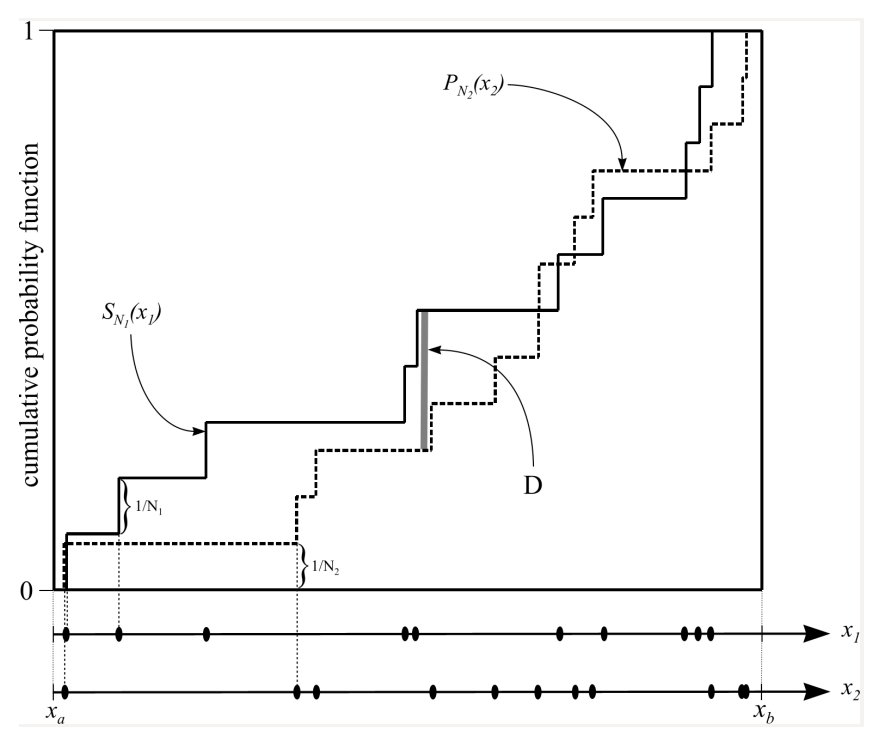
\includegraphics[height=6.9cm]{ks.eps}
   \caption{The Kolmogorov-Smirnov test}
\end{figure}
%-----------------------------------------------------------
Here an example for the way of constructing a CDF: Assume there
are $N_1=10$ measurements within a range of $[x_a,x_b]$. The data
points are shown as the quantity $x_1$ on the line labelled $x_1$
at the bottom of Fig. B.1. The cumulative distribution function
$S_{N_1}(x_1)$ is constructed by starting at $x_a$ and `moving' to
$x_b$. On every data point of $x_1$ the CDF is increased by
$1/N_1$, so it cumulates from 0 to 1 when going from $x_a$ to
$x_b$. The result is a step function. The CDF value is constant
between data points. The same is done with the theoretical
distribution $P_{N_2}(x_2)$ the data of which are shown on the
line labelled $x_2$ at the bottom of Fig. B.1. In our case
$P_{N_2}(x_2)$ is based on random distributions of $10^6$
galaxies, so it has discrete values, too. This leads to a second
step function. However it is much more smoother than the one of
the observations, because of the higher number of data.\\\\
The K-S test behaves conservative in case of a discrete
$P_{N_2}(x_2)$, so it overestimates the null hypothesis. If
$P_{N_2}(x_2)$ is based on a continuous function, this test does
not overestimate the null hypothesis.\\\\
All cumulative functions constructed in this way have two common
properties: they are zero at the beginning of their range of
definition and 1 on their end. The comparison of the two
distribution functions $S_{N_1}(x_1)$ and a continuous theoretical
$P(x)$ is done with the help of the quantity $D$, which is defined
as
%--------------------------------------
\begin{equation}
    D=\max_{x_a<x<x_b}|S_{N_1}(x)-P(x)|
\end{equation}
%--------------------------------------
So it is the largest difference between the two cumulative
functions. In case of a non-continuous $P_{N_2}(x_2)$, as used in
this work, this becomes
%--------------------------------------
\begin{equation}
    D=\max_{x_a<x<x_b}|S_{N_1}(x)-P_{N_2}(x_2)|
\end{equation}
%--------------------------------------
The quantile ($Q_{KS}$) is a function of $\lambda$ and can be
calculated by
%--------------------------------------
\begin{equation}\label{k_s}
    Q_{KS}(\lambda)=2\sum_{j=1}^\infty (-1)^{j-1}e^{-2j^2\lambda^2}
\end{equation}
%--------------------------------------
which is a monotonic function with the limiting values
%--------------------------------------
\begin{equation}
    Q_{KS}(0)=1, \quad Q_{KS}(\infty)=0
\end{equation}
%--------------------------------------
The parameter $D$ measures the maximum values of the absolute
difference between two cumulative distribution functions. In terms
of this function, the significance level of an observed value of
$D$ is given approximately (Stephens 1970) by,
%---------------------------------------
\begin{equation}
    P(D>$observed$)=Q_{KS}([\sqrt{N_e}+0.12+0.11/\sqrt{N_e}]D)
\end{equation}
%---------------------------------------
where $N_e$ is the effective number of data points, defined by
%--------------------------------------
\begin{equation}
    N_e=\frac{N_1N_2}{N_1+N_2}.
\end{equation}
%--------------------------------------
with $N_1$ denoting the number of data in the observations and
$N_2$ being the number of data in the theoretical set.\\\\
The nature of the distribution given in equation \eqref{k_s} is that it
becomes asymptotically accurate as the $N_e$ becomes $\geq$ 4
(Stephens 1970).\\\\
The K-S test tends to be most sensitive around $P(x)=0.5$, the
median value. At $P(x)=0$ or 1 it is less sensitive. The reason is
that the probability for larger $D$ is largest at the median value
of $P(x)$, because at $P(x)=0$ and $P(x)=1$ both CDFs coincide,
whereas the probability of a coincidence is smallest at the median
value of $P(x)$. So a large amount of steps in one of the CDFs can
cause a larger distance between both CDFs around $P(x)=0.5$.\\\\
\section{Kuiper-V Test}\label{kvtest}
The Kuiper-$V$ statistics (Kuiper, 1962) is a variant of the
Kolmogorov-Smirnov statistics. The basic idea is to take advantage
of the invariance of reparametrization of the $x$-axis. One can
``wrap" the $x$-axis into a circle  and look
for a statistic which is invariant under shifts.
\begin{figure}[h]\label{kv}
   \centering
   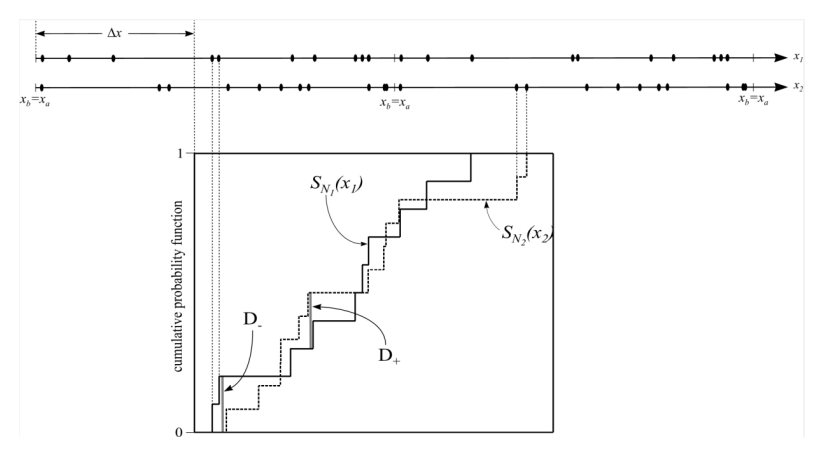
\includegraphics[height=9cm]{kuiper.eps}
   \caption{Kuiper-$V$ test: The CDF's are
   constructed in the same way like the K-S test, except the starting
   point is shifted by $\Delta x$ which leads to different CDF's. The measurement
   quantity for the Kuiper-$V$ test is the now the sum $D=D_++D_-$, the two largest
   distances above and below $S_{N_1}(x_1)$ between the two CDF's. This new quantity leads to an independence of
   the sensitivity of the test.}
\end{figure}
%----------------------------------------
The data set is the same as used in the example of the previous
chapter. Fig. B.2 shows the cumulative distribution functions
$S_{N_1}(x_1)$ and $S_{N_2}(x_2)$. It can be seen that they are
different from the one in Fig. B.1. The reason is that the starting
point is shifted by an offset $\Delta x$. The Kuiper-$V$
statistics is defined by
%--------------------------------------
\begin{equation}
\begin{array}{l}
    V=D_++D_-
    \\=\max[S_{N_1}(x)-S_{N_2}(x)]+\max[S_{N_2}(x)-S_{N_1}(x)]
\end{array}
\end{equation}
%--------------------------------------
$D_+$ and $D_-$ are the largest distances between $S_{N_1}$ and
$S_{N_2}$. $D_+$ lies above $S_{N_1}$, $D_-$ below.

The quantile ($Q_{KP}$) of the Kuiper-$V$-statistics can be
calculated by
%----------------------------------------
\begin{equation}
    Q_{KP}(\lambda)=2\sum_{j=1}^{\infty}(4j^2\lambda^2-1)e^{-2j^2\lambda^2}
\end{equation}
%----------------------------------------
which is again monotonic and has the following limits:
%----------------------------------------
\begin{equation}
    Q_{KP}(0)=1, \quad Q_{KP}(\infty)=0
\end{equation}
%----------------------------------------
The approximative function to calculate the significance level for
the disproof of the null hypothesis is given by (Stephens 1970)
%---------------------------------------
\begin{equation}
    P(V>$observed$)=Q_{KP}([\sqrt{N_e}+0.155+0.24/\sqrt{N_e}]V)
\end{equation}
%---------------------------------------
where $N_e$ represents the effective number of data points.\\\\
The trick to obtain the same sensitivity over the whole range of
definition is to take the sum of $D_+$ and $D_-$. So this
statistic becomes invariant under shifts (=variations of $\Delta
x$) (Kuiper, 1962). Therefore the sensitivity of the test is not a
function of $x$. Of course the individual values of $D_+$ and
$D_-$ vary with different starting points $\Delta x$, but the sum
stays constant (Kuiper, 1962). This property makes this test
perfect for all problems defined on circles, periods, cycles, and
so on.\\\\
The conditions for anisotropy are as follows:
chi-square probability P($>\chi^2)<$0.050, correlation
coefficient $C/\sigma(C)>$1, first order Fourier coefficient
$\Delta_{11}$/$\sigma(\Delta_{11}$)$>$1 and the first order
Fourier probability P($>\Delta_1$)$>$0.150 as used by Godlowski
(1993, 1994) K-S=1 and Kuiper-V=1. In $\theta$ distribution, a positive(negative) $\Delta_{11}$ suggests that the spin vectors of galxies tend to orient parallel  (perpendicular) to the reference coordinate system. In $\phi$-distribution, a postive (negative) $\Delta_{11}$ suggests that the spin vector projections of galaxies tend to point radially (tangentially) with respect to center of the reference coordinate system.
